%!TEX root = ../../thesis.tex
\chapter{Quantifying Reticulation Using Topological Complex Constructions Beyond Vietoris-Rips}
\label{ch:complex_construction}

\section{Introduction}
\label{complex_construction:introduction}

In Chapter~\ref{ch:background}, the Vietoris-Rips complex was introduced as a construction on molecular sequence data.
The persistent homology of a filtered sequence of complexes was shown to provide a quantitative measure of reticulate processes.
As we will show, in certain cases the Vietoris-Rips complex can have a reduced sensitivity to reticulation.
In this chapter we introduce two ideas to increase the usefulness of the signal generated by persistent homology.
The first is an approach for imputing latent ancestors into the data that increases the quantitative signal detected by persistent homology.
Our approach is built on the \emph{median graph} construction.
Median graphs form the basis for a large number of phylogenetic network algorithms and are closely related to split decompositions of finite metrics \cite{Bandelt:1999,Bandelt:1992}.
A common desire is an approach to quantify the complexity of the resulting construction.
We show that the persistent homology of the median closure is a fast and efficient way to identify the phylogenetic incompatibility in a dataset.
The second is an approach for computing \Cech\ complexes from genomic data.
The \Cech\ complex, introduced in Section~\ref{bg:tda:math:complexes}, has certain advantages over the Vietoris-Rips complex.
However, it requires a notion of embedding space for data, which for genomic data is not entirely obvious.

The structure of this chapter is as follows.
In Section \ref{complex_construction:sensitivity} we show simple examples of the reduced sensitivity of the Vietoris-Rips for detecting reticulations.
In Section \ref{complex_construction:median_complex} we introduce the median closure of the original vertex set.
We show how this operation recovers invariant signals of phylogenetic incompatibility in a quantitative way.
In Section \ref{complex_construction:cech_complex} we present a \Cech\ complex construction on sequence data.
Throughout, we assume biallelic data under an infinite sites model with no back mutation.

\section{Sensitivity of the Vietoris-Rips Construction}
\label{complex_construction:sensitivity}

The fundamental loop (00,10,01,11) was introduced in Section~\ref{bg:top4bio:fundamental_unit} as the simplest example in which binary sequence data would manifest reticulation, as measured by persistent homology.
The fundamental loop is based on the four-gamete test of haplotype incompatibility in an infinite sites model.
In considering further small examples of sequence data we often encountered situations in which the four gamete test indicated reticulate evolution, but persistent homology failed to detect a loop.
This was often due to degeneracies that would arise because of either (a) incomplete sampling in which case recombinations failed to be detected because parental and ancestral strains would collapse prior to connecting with the recombinant offspring, or (b) cases in which the recombination event led to an offspring that sat spatially intermediate to the ancestral and parental strains.
We demonstrate with two examples.

\paragraph{Example One}
\label{ex:example1}
%
It is generally the case that we do not have a complete sampling of the sequences corresponding to the evolutionary history of a set of sequences.
For example, we may not have sampled the true recombinant child, only a descendant which has accumulated additional mutations.
Consider the set of sequences 000, 100, 010, and 111.
From the four-gamete test we know there is an incompatibility between sites 1 and 2, indicating the presence of a reticulate event.
Let us arbitrarily choose $s_1$ to be the common ancestor, $s_2$ and $s_3$ to be parents, and $s_4$ to be a descendant of the reticulate event.
We can infer that the recombinant was of the form $s_r=110$.
Unfortunately, the persistent homology the four sequences will be trivial.
To understand why, consider an embedding of the four sampled sequences onto the 3-cube, as seen in Figure XXX.

The failure to detect the loop is due to the ancestral and parent sequences collapsing before connecting with the recombinant child.
In general, for a loop to be detected, the two internal distances must be greater than any of the four side distances.
In this case, the internal distance from parent 1 ($s_2$) to parent 2 ($s_3$), $d_{23}$ is equal to the distances from each parent to the sampled descendant of the recombinant ($d_{24}$ and $d_{34}$).
This is a general issue with the application of the Vietoris-Rips complex to phylogenetic data.

\paragraph{Example Two}
\label{ex:example2}
%
This example is taken from \citet{Song:2005}.
Consider the set of sequences: $s_{1}=0000$, $s_{2}=1100$, $s_{3}=0011$, $s_{4}=1010$, and $s_{5}=1111$.
There are pairwise incompatibilities between sites $1$ and $3$, $1$ and $4$, $2$ and $3$, and $2$ and $4$.
Performing the Hudson-Kaplan test yields $R_M=1$, with a partition between sites 2 and 3.
\citet{Song:2005} showed that a minimum of two recombinations were required to explain this data.
In this example, persistent homology will contract immediately, with trivial higher homology.
To understand why this is the case, consider an embedding into $\mathbb{R}^3$.
The problem is that $s_{3}$ sits in the middle of the other four sequences, and at $\epsilon=2$ everything contracts.
Had $s_{3}$ not been present in the data, we would have had an example very similar to Example \ref{ex:example1}, with the interpretation of one recombination event.
We term this the ``dixie cup'' example.
The conclusion to draw from this example is that multiple recombination events can interact in complicated ways, destroying signal from persistent homology.

\begin{figure}
\centering
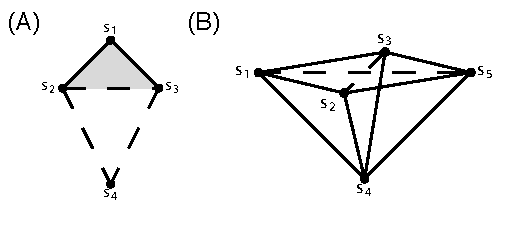
\includegraphics[width=\columnwidth]{./fig/complex_construction/simple_examples_1.pdf}
\caption[Two examples of reduced sensitivity of the Vietoris-Rips Complex]{Two examples in which the standard filtration fails to identify reticulate evolution. (A) In this example, the ancestral sequences collapse before forming a loop with the recombinant offspring. (B) In this example, multiple recombinations interact to create a degeneracy, and the entire complex collapses immediately. (From Song and Hein \cite{Song:2005})}
\label{fig:complex_construction:simple_examples}
\end{figure}

\section{The Median Complex Construction}
\label{complex_construction:median_complex}

The median complex is an alternative construction on sequence data aimed at recovering signal of phylogenetic incompatibility using homology.
First, we define the median of a set of aligned sequences.

\begin{defn}
  \label{defn:median}
  For any three aligned sequences $a$, $b$, and $c$, the \emph{median} sequence $m(a,b,c)$ is defined such that each position of the median is the majority consensus of the three sequences.
\end{defn}

For example, consider the three sequences $a=110$, $b=011$, and $c=101$.
At each site we have the set $\{1,1,0\}$.
The majority consensus for each site is $1$, therefore the median sequence is $m=111$.
In any further analysis, we augment the original data to include the computed median sequence.
Note that as defined here, the median operation is defined only for binary sequences.

\begin{figure}
\centering
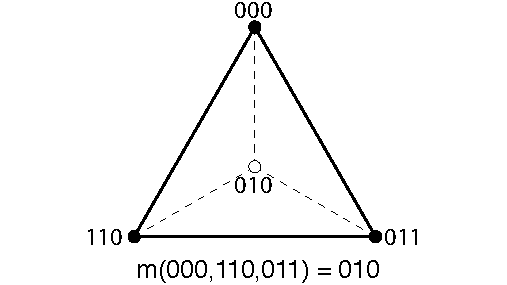
\includegraphics[width=.75\columnwidth]{./fig/complex_construction/median.pdf}
\caption[The Median Operation on Binary Sequences]{The median is defined as the majority allele at each position. The median closure imputes the median into the original vertex set.}
\label{fig:complex_construction:median}
\end{figure}

Having defined the median operation, we now define the \emph{median closure}.
Given an alignment $S$, the median closure, $\bar{S}$, is defined as the vertex set generated from the original set $S$ that is closed under the median operation,
\begin{equation}
\bar{S} = \{v \colon v=m(a,b,c) \in \bar{S} \forall a,b,c \in \bar{S}\}
\end{equation}
We can obtain the median closure $\bar{S}$ by repeatedly applying the median operation to sets of three sequences until no new sequences are added.
Effectively, computing the median closure imputes interior nodes into the dataset.
We call complexes formed from the original sequences the \emph{leaf complexes}, and call complexes formed from the median closure the \emph{median complexes}.
We can then proceed by computing the persistent homology of this median closure.
The downside of the median closure operation is that we can no longer identify the loops we measure as reticulate events.
The median closure operation can generate multiple loops from a single incompatibility.
We now revisit our two examples.

\emph{Example 1.}
One median vertex, $m(s_2,s_3,s_4)=110$, as shown in Figure~\ref{fig:example_1_revisited}.
This vertex, labeled $s_r$, acts as the recombinant offspring of $s_2$ and $s_3$.
Persistent homology now detects an $H_{1}$ loop in the range $\epsilon=[1,2)$ formed between $s_1$, $s_2$, $s_3$, and $s_r$.
$s_4$ is interpreted the descendant of $s_r$.

\begin{figure}
\centering
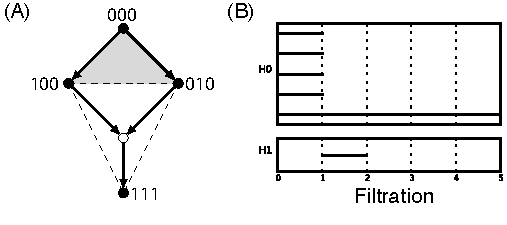
\includegraphics[width=\columnwidth]{fig/complex_construction/example_1_revisited.pdf}
\caption[The Median Complex Recovers Reticulation in Example One]{One median node (white node), which acts as the recombinant offspring of $s_2$ and $s_3$. One $H_1$ loop detected in the interval $[1,2)$.}
\label{fig:example_1_revisited}
\end{figure}

\emph{Example 2.}
Four median vertices, as shown in Figure~\ref{fig:example_2_revisited}.
Persistent homology now detects four $H_{1}$ intervals in the range $\epsilon=[1,2)$.
In this case, the median closure now overestimates the minimum number of recombinations required.
This example shows a potentially complicating aspect of the median closure in that specific $H_1$ features are no longer identifiable with specific reticulate events.

\begin{figure}
\centering
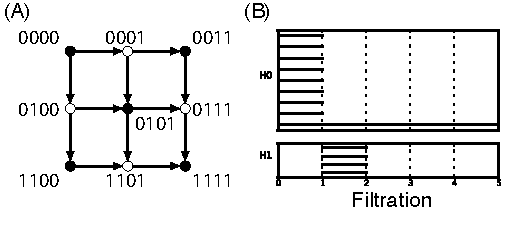
\includegraphics[width=\columnwidth]{fig/complex_construction/example_2_revisited.pdf}
\caption[The Median Complex Recovers Reticulation in Example Two]{Four median vertices (white nodes). Four $H_1$ loops now detected in the interval $[1,2)$.}
\label{fig:example_2_revisited}
\end{figure}

Filtrations on Buneman graphs have been defined previously \citep{Dress:1997}, but not using an explicit sequence representation.
They have been defined in terms of the split decomposition, which is a deconstruction of the data into sets of possibly-conflicting bipartitions.\footnote{In a tree, each edge defines a bipartition, or split. A reticulate history will be characterized by incompatible splits.}
The filtration defined in \citet{Dress:1997} is based on a complicated polytope construction scheme defined directly from the split decomposition.
Given that all median graphs are split networks \citep{Huson:2010}, the constructions are identical but the extracted information is not.
To the best of our knowledge, quantification of the complexity of these objects has not been measured using homological tools.

\subsection{Inclusion}
%
We have examined the persistent homology of two topological constructions on sequence data: the leaf complex and the median complex.
Counting $\beta_1$ intervals in the leaf complex underestimates reticulate evolution because of incomplete sampling, while counting $\beta_1$ intervals in the median complex overestimates reticulate evolution.
The median complex is in some sense an upper bound on probable recombination histories, and contains within it all possible recombination graphs within it (not strictly true, as there are infinitely many complicated ARGs - but it does contain within it all maximum parsimony trees).
We can hypothesize that there exists a true complex, called the \emph{evolutionary complex}, which will accurately reflect the evolutionary relationships in the sequences.
Information about the evolutionary complex is not available to us, however we can say that there exists an inclusion between the homotopy types of the three complexes

\begin{equation}
 \mathrm{Cl}(\mathcal{LC}) \hookrightarrow \mathrm{Cl}(\mathcal{EC}) \hookrightarrow \mathrm{Cl}(\mathcal{MC})
\end{equation}

Recovery of an optimal $\mathcal{EC}$ is the task of many ARG-based methods and is known to be an NP-hard problem and is not considered here.
For example, given an $\mathcal{EC}$ as computed from some other tool, we might be able to say something useful about the topological complexity.

\subsection{Phylogenetic Examples}

Here we consider two standard datasets from the phylogenetics literature.
In both examples, the standard filtration yielded no higher homology.
We generated the median closure and computed homology on that.
Datasets are represented using a triangle-free network construction, which approximates the computed homology.

\subsubsection{{\textit{D. melanogaster}} Data}

A benchmark dataset in studying recombination is the Kreitman data \cite{Kreitman:1983}.
The dataset consists of eleven sequences (nine unique) of the Adh locus from \emph{Drosophilia melanogaster} collected from various geographic locations, with 43 segregating sites.
The Hudson-Kreitman test yields 6 reticulate events.
Computing the median closure expands the dataset to 46 vertices.
Here we have non-trivial homology: 32 $H_1$ loops and 3 $H_3$ loops.
In the visualized network, the complex reticulations ($H_3$) are localized to the bottom-most samples.
The $H_1$ reticulations, on the other hand, are not very localized and persist across geographic regions.
The barcode plot is shown in Figure~\ref{fig:kreitman}.

\begin{figure}
\centering
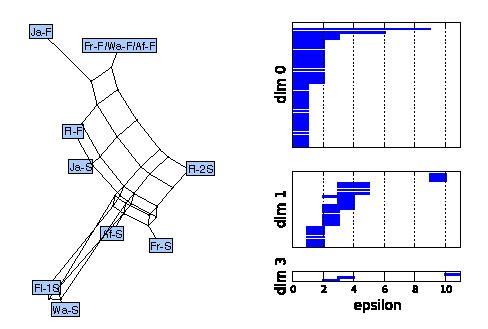
\includegraphics[width=\columnwidth]{fig/complex_construction/kreitman.pdf}
\caption[Recombination in \emph{D. melanogaster}]{Recombination in \emph{D. melanogaster}. Persistent homology identifies several complex reticulations in the population.}
\label{fig:kreitman}
\end{figure}

\subsubsection{{\textit{Ranunculus}} Data}

Natural hybridization occurs frequently in plants.
Here we examine reticulation in the maturase K (matK) protein in nine species from genus \emph{Ranunculus}.
This data is originally from \cite{Huber:2001vv}.
From nine initial species, the median closure has 32 vertices.
Persistent homology is computed and the barcode diagram shown in Figure~\ref{fig:buttercup}.
Looking at $H_0$, we identify two clusters of species.
Further, we identify 17 $H_1$ loops and 3 $H_3$ loops.
Comparing with the \emph{D. melanogaster} data, reticulation at this locus is both smaller in scale (shorter bars at small filtration values) and less frequent (fewer total bars).
Additionally, the complex reticulations are localized within each $H_0$ cluster.

\begin{figure}
\centering
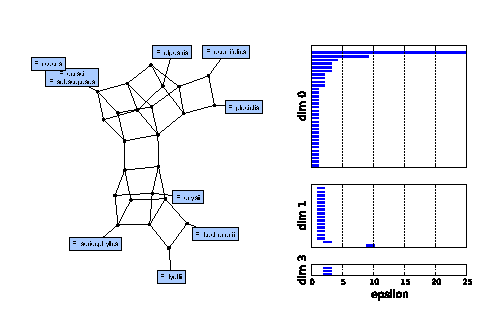
\includegraphics[width=\columnwidth]{fig/complex_construction/buttercup.pdf}
\caption[Species hybridization in genus \emph{Ranunculus}]{Species hybridization in genus \emph{Ranunculus}. Persistent homology identifies two populations separated by complex reticulations.}
\label{fig:buttercup}
\end{figure}

\section{\Cech\ Complex Construction as an Optimization Problem}
\label{complex_construction:cech_complex}

The \Cech\ complex is defined on a set of points $S$ as
\begin{equation}
\mathrm{\check{C}ech}(r) = \left\{\sigma \subseteq S | \bigcap_{x\in\sigma} B_x(r) \neq \emptyset \right\},
\end{equation}
where $B_x(r)$ is the ball of radius $r$ centered at vertex $x$.
By the nerve lemma, the homotopy type of the \Cech\ covering is guaranteed to be identical to that of the original topological space \citep{Borsuk:1948}.

Computing the \Cech\ complex is often an expensive operation, such that in practice the Vietoris-Rips complex is used.
Unlike the Vietoris-Rips complex, which is entirely defined by the 1-skeleton, the \Cech\ complex requires one to check each simplex $\sigma$ up to some maximum dimension $D$.
The \Cech\ complex therefore requires one to know the ambient space the data is embedded in, unlike a Rips complex which can be built directly from distance data.
Binary sequence data of length $d$ explicitly sits on the discrete lattice of $\{0,1\}^d$ with an $L_1$ norm.
In this case, it is not immediately obvious how to define when three sequences should form a simplex.
One
Therefore, we expand the ambient space to $\mathbb{R}^d$ with an $L_1$ metric.
This choice of metric is motivated by two reasons.
First, the $L_1$ norm maintains the Hamming distance between sampled points.
Second, the $L_1$ norm keeps the primary theorem intact, that is tree like data generates trivial homology.
\footnote{This notion has a natural extension to multiallelic sites which is not detailed here.}

The problem of deciding if a particular simplex $\sigma$ belongs in the \Cech\ complex at radius $r$ is the same as checking if a ball of radius $r$ can be placed such that each point $x$ in $\sigma$ is contained within the ball.
In $\mathbb{R}^d$ with an $L_2$ metric there exists an efficient randomized algorithm for computing this radius known as the \emph{miniball algorithm}.\autocite{Gartner:1999}
However, the efficiency of the miniball algorithm relies on the strict convexity of the $L_2$ metric and therefore is not applicable to a space with an $L_1$ metric.
Instead, we pose the miniball problem in $L_1$ as a generic convex optimization problem, and use standard library solver.
That is, we define a $d+1$ dimensional optimization problem where $x$ is the miniball center and $R$ is the miniball radius.

The problem is stated as
\begin{align*}
\text{minimize}\qquad   &  R \\
\text{subject to}\qquad & \forall p \in P: ||x-p||_{1} \leq R \\
                        & x \in \mathbb{R}^d
\end{align*}

We implement the problem in \texttt{cvxpy}.
\kje{TODO: A brief comment about the complexity of this routine.}
The randomized miniball algorithm has constant complexity in dimension.

\subsection{Molecular Hypothesis}

Gromov proved that a median graph is the 1-skeleton of a CAT(0) cubical complex \citep{Gromov:1987}.
The homology of a cubical complex can be efficiently computed using the methods of \citet{Kaczynski:2004} through a slightly different construction.
We define a cubical flag complex and build a filtration dimension by dimension (to expand on this point...)
The barcode diagram will then have the natural interpretation of being composed of sets of hypercubes of varying dimension.
If we consider each bar of dimension $n$ in the barcode diagram in turn, we can determine the incompatible sites that it represents.
Dimension $1$ bars ($2$-cubes) will have one pair of incompatible sites with four haplotypes.
Dimension $2$ bars ($3$-cubes) will have three pairs of incompatible sites with eight haplotypes.
In general, $n$ bars will represent $n+1$-cubes in which all $2^{(n+1)}$ haplotypes are present in the vertices of the generating cycle.

From the barcode diagram it will not in general be possible to decompose our construction into the primitive building blocks of hypercubes.
This is because the hypercubes of dimension ($n>2$) will in general not be independent, but can interact by sharing lower dimensional faces.
Nonetheless, to aid in decomposing the barcode diagram, we constructed the following table, which contains the homology ranks (betti numbers) for powers of the hypercube graph, computed using the \Cech\ complex.
Incidentally, it was understanding the structure of numbers in a table very much like Table \ref{table:hypercube_homology} which led us to find a method of computing Cech homology instead of Rips homology.

\begin{table}
\centering
\caption{\Cech\ Homology of Hypercube}
\begin{tabular}{lcccccc}
\toprule
$d=$    & 1 & 2 & 3 &  4 &  5 &   6\\
\midrule
$H_{0}$ & 2 & 4 & 8 & 16 & 32 &  64\\
$H_{1}$ & 0 & 1 & 5 & 17 & 49 & 129\\
$H_{2}$ & 0 & 0 & 1 &  7 & 31 & 111\\
$H_{3}$ & 0 & 0 & 0 &  1 &  9 &  49\\
$H_{4}$ & 0 & 0 & 0 &  0 &  1 &  11\\
$H_{5}$ & 0 & 0 & 0 &  0 &  0 &   1\\
$H_{6}$ & 0 & 0 & 0 &  0 &  0 &   0\\
\bottomrule
\end{tabular}
\label{table:hypercube_homology}
\end{table}

We include a simple proof of the numbers in this table [right here].

% \subsection{Simple Examples}
% \label{subsec:higher_dim_examples}
% %
% Generation of one dimensional homology requires the presence of four incompatible haplotypes (00, 10, 01, 11).
% That is, there is a condition on pairs of segregating sites, and at least two sites will be required to generate $H_1$.
% Homology of dimension $n>1$ will be a higher order effect and require the interaction of multiple pairs of sites.
% One might surmise that all possible haplotypes on $n$ segregating sites are required to generate homology of dimension $n-1$.
% For example, on the 3-cube, there are eight haplotypes.
% $H_2$ is generated in the interval $[1.0,1.5)$.

% In fact, subsets of the 3-cube generating $H_2$ can be formulated.
% Consider the set of sequences $S=(000,100,010,001,111)$.
% The persistent homology of $S$ will generate $H_2$ in the interval $[1,1.5)$.
% A possible evolutionary scenario is presented in Figure XXX.
% We see that sequence $s_5$ is a triple reassortment of sequences $s_2$, $s_3$, and $s_5$.
% Further, notice that there is total incompatibility between sites $(1,2)$, $(2,3)$, and $(1,3)$.
% Contrast this with the example detailed in Figure XXX.
% Here, we have a set of six sequences which exhibits two $H_1$ loops, and no $H_2$ homology.
% The two loops can be seen as independent.
% And if we examine

\section{Conclusions}
\label{complex_construction:conclusion}

Persistent homology can capture and quantify complex patterns of reticulation in genomic data.
The standard Vietoris-Rips filtration is susceptible to reduced sensitivity due to incomplete sampling or interactions between reticulations.
Constructing the median closure of the original sequence set increases the topological signal of reticulation.
Future work will focus on efficient implementations of constructing this closure.
We also introduced a \Cech\ complex construction on genomic data.
The construction treats filling higher-dimensional simplices as an optimization problem, which is solved using the miniball algorithm.
An interesting additional observation is that the number of recombinations required to explain the fully saturated hypercube is exactly equal to the alternating sum of the homology ranks.